\documentclass[table]{beamer}
\usepackage[french]{babel}
\usepackage{tikz}
\usepackage[utf8]{inputenc}
\usepackage[T1]{fontenc}

\usepackage{beamerthemesplit}
\usetheme{AnnArbor}
\usecolortheme{beaver}
\usefonttheme{professionalfonts}


\usepackage{wasysym}
\usepackage{times}
\usepackage{subfigure}
\usepackage{fancyvrb}
\usepackage{booktabs,multirow,rotating, tabularx}
\usepackage{graphicx}
\usepackage{listings}

\lstset{ 
  captionpos=b,                    % sets the caption-position to bottom
  basicstyle=\scriptsize,        % the size of the fonts that are used for the code
  breaklines=true,                 % sets automatic line breaking
%  numbers=left,                    % where to put the line-numbers; possible values are (none, left, right)
%  numbersep=5pt,                   % how far the line-numbers are from the code
%  numberstyle=\tiny\color{mygray}, % the style that is used for the line-numbers
  rulecolor=\color{black},         % if not set, the frame-color may be changed on line-breaks within not-black text (e.g. comments (green here))
  showspaces=false,                % show spaces everywhere adding particular underscores; it overrides 'showstringspaces'
  showstringspaces=false,          % underline spaces within strings only
%  stepnumber=2,                    % the step between two line-numbers. If it's 1, each line will be numbered
  tabsize=2,	                   % sets default tabsize to 2 spaces
  title=\lstname,                   % show the filename of files included with \lstinputlisting; also try caption instead of title
  inputencoding=utf8,
  literate={é}{{\'e}}1 {ê}{{\"e}}1 {è}{{\`e}}1 {î}{{\^i}}1 {à}{{\`a}}1 {ù}{{\`u}}1 {ç}{{\c c}}1 
}

%------------------------------------------------------------------------------------

\hypersetup{
    pdfauthor   = {Romuald THION},%
    pdftitle    = {DIU-EIL Bloc 4},%
    pdfsubject  = {Le modèle relationnel},%
    pdfkeywords = {DIU, bases de données, algèbre relationnelle},%
    colorlinks  = false,
    linkbordercolor = blue, % hyperlink borders will be red
    pdfborderstyle = {/S/U/W 1}% border style will be underline of width 1pt
}	

\title[DIU-EIL Bloc 4 -- SD]{
    \textsc{DIU-EIL Bloc 4\\ Structures de données}
}

\author[R. THION, N. PRONOST]{
    Romuald THION, Nicolas PRONOST
}
\institute{ 
{  
    \url{https://forge.univ-lyon1.fr/diu-eil/bloc4}}
}

%\date{Mardi 21 juin 2011 (matin)}

\newcommand{\bleu}[1]{{\color{cyan} #1}}
%-------------------------------------------------------------------------------

\usefoottemplate{%
  \vbox{% 
    \tinycolouredline{black}%
      {\color{white}\insertshortauthor\hfill\insertshorttitle\hfill\insertframenumber}%
}}

%\usefoottemplate{}

\setbeamertemplate{navigation symbols}{}
\beamertemplatetransparentcovereddynamicmedium 

%\AtBeginSection[]{
%  \begin{frame}%{Sommaire}
%  \tableofcontents[currentsection, hideothersubsections]
%  \end{frame} 
%}




\begin{document}
	\begin{frame}
		\titlepage
	\end{frame}

    \begin{frame}{Plan}
        \tableofcontents[hideallsubsections]
    \end{frame} 

%%%%%%%%%%%%%%%%%%%%%%%%%%%%%%%%%%%%%%%%%%%%%%%%%%%%%%%%%%%%%%%%%%%%%%%%%%%%%%%%
\section{Présentation générale}
%%%%%%%%%%%%%%%%%%%%%%%%%%%%%%%%%%%%%%%%%%%%%%%%%%%%%%%%%%%%%%%%%%%%%%%%%%%%%%%%


\begin{frame}{Positionnement programme NSI}
  
    \begin{figure}
      \centering
      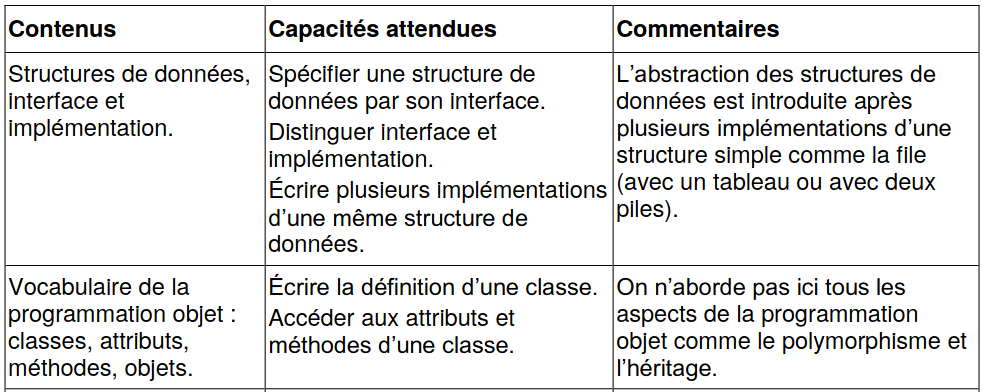
\includegraphics[width=0.9\linewidth]{./NSIa.png}%
    \end{figure}
\end{frame}


\begin{frame}{Positionnement programme NSI}
  

    \begin{figure}
      \centering
      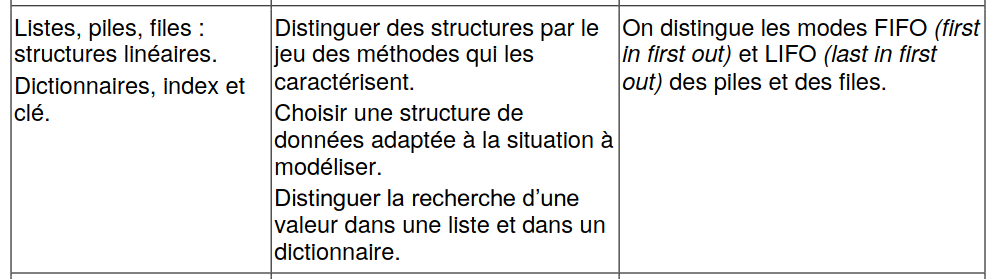
\includegraphics[width=0.9\linewidth]{./NSIb.png}%
    \end{figure}
  
  \begin{center}
    \emph{Les autres structures (arbres, graphes) étant dans le bloc 5}
  \end{center}
  
\end{frame}


\begin{frame}{Définition générale}
  
  \begin{block}{Extrait de \href{https://en.wikipedia.org/wiki/Data_structure}{Wikipedia}}
  \begin{quote}
    In computer science, a data structure is a data \emph{organization}, \emph{management}, and \emph{storage} format that enables \alert{efficient access and modification}. [\ldots] Data structures serve as the basis for abstract data types (ADT). The ADT defines the \alert{logical form} of the data type. The data structure \alert{implements the physical form} of the data type.    
  \end{quote}
  \end{block}

\end{frame}

\begin{frame}{Type abstrait VERSUS structure de données}

  On peut différencier 
  \begin{itemize}
    \item Le \alert{type abstrait} : les opérations et les propriétés qui les lient
      \begin{itemize}
        \item notion d'interface (en POO), de spécification, d'API
        \item \emph{e.g.,  \texttt{p.push(x); p.pop()} laissent une pile \texttt{p} inchangée}
      \end{itemize}
    \item La \alert{structure de données} : une implantation physique qui réalise cette spécification
    \begin{itemize}
      \item ce qui va compter c'est la performance (évaluée en moyenne ou au pire cas) des opérations
      \item \emph{e.g., un tableau dynamique, une liste doublement chainée, etc.}
    \end{itemize}

  \end{itemize}


\end{frame}



\begin{frame}{Interface de liste (simplement chainée)}

  \lstinputlisting[language=Python]{./Liste.py}
\end{frame}


\begin{frame}{Type abstrait VERSUS structure de données}


%\pause

\begin{center}
  \alert{Attention} :\emph{ pour un type abstrait, on peut avoir plusieurs implantation avec des structures de données différentes !}
\end{center}

\pause
\begin{center}
  \alert{Attention} : \emph{pour un type abstrait, on \og{}s'attend\fg{} souvent à avoir les performances d'une certaine structure, ce qui peut-être contre-intuitif\\
  Exemple typique : le type \texttt{list} de Python}
\end{center}



\end{frame}




\begin{frame}{Tableau de synthèse}

\begin{center}
  Réaliser un logiciel consiste à, notamment, choisir \alert{les structures de données adaptées} pour résoudre le problème posé.
\end{center}


    \begin{figure}
      \centering
      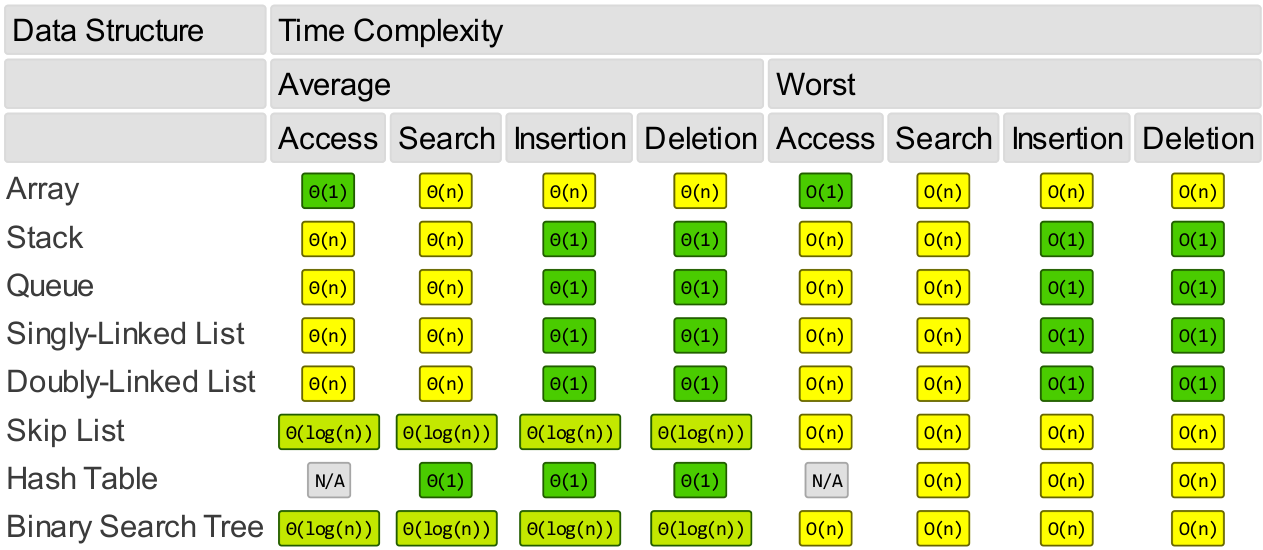
\includegraphics[width=0.9\linewidth]{./bigocheatsheet.png}%
      \caption{\url{https://www.bigocheatsheet.com/}}
    \end{figure}
  
\end{frame}


\begin{frame}{Les contenus sur cette partie du programme}
  
\begin{center}
    \url{https://forge.univ-lyon1.fr/diu-eil/bloc4/-/tree/master/2_structures_de_donnees}
    
    En TD/TP :  vous allez réaliser les principales structures de données en programmation orientée objet \alert{sans utiliser les bibliothèques} : on fait tout \emph{from scratch}
    
\end{center}
  

  
\end{frame}


%\begin{lstlisting}

%\end{lstlisting}


\end{document}
